%gibt an: Papierformat, Schriftgröße
\documentclass[a4paper,english,12pt]{article}
\setlength{\parskip}{0.2cm}
\setlength{\parindent}{0cm}
%-----------------------------------------------------------------------------------------------------------------------------
%Übersetzung von E in D
\usepackage[english]{babel} %changed to English
%Einstellung der Randabstände
\usepackage[lmargin={3.5cm},rmargin={2.5cm},tmargin={2.5cm},bmargin={2cm}]{geometry}
%zur Einbindung von Graphiken
\usepackage{graphicx}
%Bearbeitung von Kopf- und Fusszeile
\usepackage{fancyhdr}
%Schriftart
\usepackage{helvet}
%stellt unabhängige Textmarken zu Verfügung
\usepackage{extramarks}
%aktiviert eine Umgebung in der der Mathematikmodus aktiv ist
\usepackage{amsmath}
%aktiviert eine Umgebung in der der Mathematikmodus aktiv ist
\usepackage{amsthm}
%aktiviert eine Umgebung in der der Mathematikmodus aktiv ist
\usepackage{amssymb}
%aktiviert Hyperlinks
\usepackage{hyperref}
%Stellt das Eurozeichen € zu Verfügung
\usepackage[right]{eurosym}
%Übersetzt die Tastatureingaben für LaTex
\usepackage[latin1,utf8]{inputenc}
\usepackage{fancybox}
\usepackage[dvipsnames]{xcolor} %more pre-defined colors
\usepackage{color}
\usepackage{colortbl} %colors in tables for horizontal and vertical lines
\definecolor{myorange}{RGB}{247,150,0} %colors from ppt graphics for uniform coloring
\definecolor{mygreen}{RGB}{0,150,130} %KIT green/blue
\definecolor{myred}{RGB}{192,80,77}
\definecolor{myblue}{RGB}{79,129,189}
\usepackage{float}
\usepackage{framed}
\usepackage{url}
\usepackage{verbatim} %multi-line comments
\usepackage[titles]{tocloft} %toc design

% \usepackage[utf8]{inputenc}

% \usepackage[square,sort,comma,numbers]{natbib}
\usepackage{natbib}

\usepackage{booktabs}
\usepackage{tabularx} %Tabellen, die sich der Seitenbreite anpassen

\usepackage{multirow} % Verbundene Zellen in Tabellen
\usepackage{rotating} % Quergestellte Tabellen
\usepackage{rotfloat}

\usepackage[bottom]{footmisc} %Fußnoten immer am Ende der Seite
\usepackage{tikz} %for graphics, eg trees
\usepackage{tcolorbox} %color for graphics
\usepackage{pgfkeys}
\usepackage{multicol} %multi-column
\usepackage{colortbl} % colour of table lines
\usepackage{algorithm}
\usepackage{algpseudocode}
\usepackage{algorithmicx} %layout for algorithms
\usepackage{xfrac} %layout for fractions

%%% MY PACKAGES
\usepackage{lineno,hyperref}
\usepackage{booktabs} % for loading .txt files into this document
\usepackage{amsmath}
\usepackage{eurosym} % for the euro sign
\modulolinenumbers[5]
% \usepackage[disable]{todonotes} % for hiding the todo notes
\usepackage[colorinlistoftodos,prependcaption,textsize=small]{todonotes}
\usepackage{graphicx} % für bullet points?

%%%
%Definitionen
\newtheoremstyle{mystyle}% name
{10pt}% Space above
{10pt}% Space below
{\itshape}% Body font
{}% Indent amount:
{\bfseries}% Theorem head font
{:}% Punctuation after theorem head
{0.5em}% Space after theorem head
{\thmname{#1}\thmnumber{ #2}:\thmnote{ #3}}% Theorem head

\theoremstyle{mystyle}% default
\newtheorem{definition}{Definition}
\numberwithin{equation}{section}
\renewcommand{\proofname}{Beweis}


%Paragraphen

\newcommand{\myparagraph}[1]{\paragraph{}\mbox{}\\}


%-----------------------------------------------------------------------------------------------------------------------------------------
\renewcommand{\baselinestretch}{1.24}
\fancyhead[LO]{\slshape \small \firstleftmark}
\fancyhead[RO]{\normalsize\thepage} \fancyfoot{}
\begin{document}
%-----------------------------------------------------------------------------------------------------------------------------------------
%Titelseite
\begin{titlepage}
% font / Schriftart
%------------------



\begin{figure}[htbp]
  %\centering

  \begin{minipage}[b]{.4\textwidth}
    
\includegraphics[width=4cm]{0_Logos/kit.jpg}
  \end{minipage}%
  \hfill
  \begin{minipage}[b]{.6\textwidth}
	\begin{flushright}
	    
\includegraphics[width=3cm]{0_Logos/IISM_logo.png}
	    \hspace{0.3cm}
        
\includegraphics[width=2.5cm]{0_Logos/KSRI_logo.png}
	\end{flushright}
  \end{minipage}

\end{figure}

\vspace*{1cm}
\begin{center}
		\LARGE{Untapping Analytical Synergies in Industrial SME Ecosystems: An Empirical Evaluation of Federated Machine Learning} %\Huge
		\vspace*{1.5cm}\\
		\large{Master Thesis}\\ %\Large
		\large{by}\\ %\Large
		\vspace*{1cm}
		\LARGE{Anna Hensel}\\ %\huge
		\normalsize{Matriculation number: 1968725}\\ %\large
		\vspace*{1cm}
		\large{ %\Large
			At the Department of Economics and Management
			\\ \vspace*{1cm}
			Digital Service Innovation (DSI)
			\\ \vspace*{0.5cm}
			Karlsruhe Service Research Institute (KSRI) \& \\
			Institute of Information Systems and Marketing (IISM)
		}
	\end{center}
	\vspace*{0.75cm}
\large{ %\Large
\begin{center}
\begin{tabular}[ht]{l c l}
  Advisor: & \hfill  &Prof. Dr. Gerhard Satzger\\
  Second Advisor: & \hfill  &Prof. Dr. Hansjörg Fromm\\
  Supervisors: & \hfill  &M.Sc. Jakob Schöffer \&\\
  \mbox{} & \hfill  &Dr.-Ing. Niklas Kühl\\
 % \mbox{} & \hfill	&Name\\
  Date of Submission:  & \hfill  & 29 October 2021\\
\end{tabular}
\end{center}
}


\vspace*{1.0cm}
	\tiny{KIT -- The Research University in the Helmholtz Association} \hfill \small{\textbf{www.kit.edu} }
\end{titlepage}


\thispagestyle{empty}\cleardoublepage

\mbox{}\thispagestyle{empty}
\cleardoublepage

{\Large \textbf{Declaration of Academic Integrity}}

\bigskip
I hereby confirm that the present thesis is solely my own work and that if any text passages or diagrams from books, papers, the Web or
other sources have been copied or in any other way used, all references---including those found in
electronic media---have been acknowledged and fully cited. \\

% "Declaration of originality:
% I hereby declare that I have composed this paper by myself and without any assistance other than the sources given in my list of works cited. This paper has not been submitted in the past or is currently being submitted to any other examination institution. It has not been published. All direct quotes as well as indirect quotes which in phrasing or original idea have been taken from a different text (written or otherwise) have been marked as such clearly and in each single instance under a precise specification of the source.I am aware that any false claim made here results in failing the examination."



\vspace{1cm}

\textit{Karlsruhe, 29 October 2021} \hspace{4cm} \textit{NAME} \\


\thispagestyle{empty}\cleardoublepage

{\Large \textbf{Abstract}}

\bigskip

Small and medium-sized enterprises (SMEs), which play a vital role in the economy, especially in Germany, increasingly want to make use of machine learning (ML), but face two major challenges: the lack of knowledge and the lack of sufficient amounts of data for training adequate models. In this work, we empirically show that federated machine learning (FL) can help SMEs with related ML use cases overcome these problems by making use of the joint data of all SMEs taking part in the federation while preserving privacy. We identify and analyze three dimensions regarding which we assess the effectiveness of FL in the SME context: \emph{performance}, \emph{privacy}, and \emph{complexity}. For the \emph{performance} dimension, we provide a simulation pipeline that lets us simulate realistic FL scenarios. We find that, regarding \emph{performance}, all SMEs potentially profit from taking part in the federation and that SMEs with a particularly challenging data situation tend to profit the most. Regarding \emph{privacy}, as only model weights are exchanged, we note that privacy requirements are usually fulfilled -- despite there being potential privacy attacks. We argue that these attacks are limited in power in common SME FL contexts and might be avoidable using basic defense strategies. Regarding \emph{complexity}, we argue that implementation and organizational complexity are crucial in the SME context, as opposed to computational complexity, which is more critical in other use cases.


\mbox{}\thispagestyle{empty}
\cleardoublepage
\rmfamily \pagestyle{fancy} \setcounter{secnumdepth}{4}


\pagenumbering{roman}
\setcounter{page}{4}
\setlength\cftparskip{-5pt}
\setlength\cftbeforesecskip{-1pt}
\setlength\cftaftertoctitleskip{-10pt}
\tableofcontents
\cleardoublepage
\phantomsection
\addcontentsline{toc}{section}{Acronyms} %include in toc w/o numbering

\markboth{ACRONYMS}{Acronyms}
\section*{Acronyms}
\begin{table}[H]
    \begin{tabular}{p{4cm} p{10cm}}
     % ACM & Association for Computing Machinery \\
     % ADA & Advanced Data Analytics \\
     AD & All Data \\
     AI & Artificial Intelligence \\
     AUC & Area under the Curve \\
     CNN & Convolutional Neural Network \\
     DLG & Deep Leakage from Gradients \\
     FedAvg & FederatedAveraging \\
     FL & Federated (Machine) Learning \\
     GAN & Generative Adversarial Networks \\
     MIA & Model Inversion Attacks \\
     ML & Machine Learning \\
     NN & Neural Network \\
     OMPC & One Model per Client \\
     PG & Performance Gain \\
     ReLU & Rectified Linear Unit \\
     RNN & Recurrent Neural Network \\
     ROC & Receiver Operating Characteristic \\
     SGD & Stochastic Gradient Descent \\
     SME & Small and Medium-Sized Enterprise \\
     TFF & TensorFlow Federated \\
    \end{tabular}%
\end{table}%


\cleardoublepage
\phantomsection
\addcontentsline{toc}{section}{List of Figures} %include in toc w/o numbering
\listoffigures
\cleardoublepage
\phantomsection
\addcontentsline{toc}{section}{List of Tables} %include in toc w/o numbering
\listoftables
\cleardoublepage

\setcounter{page}{2} \pagenumbering{arabic}

\interfootnotelinepenalty=10000 % Keine Seitenumbrüche bei Fußnoten

 % % % % % % % % % % % % %INHALTE % % % % % % % % % % % % % %

\section{Introduction\label{sec:introduction}}
% Anführungszeichen `` ''
Small and medium-sized enterprises (SMEs) play a central and distinct role for economies all over the world \citep{lukacs2005economic}.
%
Especially in Germany, where SMEs account for over half of the economic output, they are a vital driver for innovation and technology \citep{bmwi2020mittelstand}.
%
Currently, SMEs are facing major challenges concerning digitalization and the use of machine learning (ML), failing to unlock their potential.
%
Recent research using data from the Leibniz Centre for European Economic Research collected in 2019 reveals that less than 5\% of German SMEs (up to annual revenue of \euro 50 million) have applied artificial intelligence (AI) technologies in their business models so far, which stands in strong contrast to over one third of giant corporations (annual revenue larger than \euro 1 billion) having applied AI technologies \citep{hbr2021midsizeAI}.
%
Regarding the use of ML, for example for predictive maintenance and automation, SMEs often encounter two major issues.

Firstly, SMEs often lack the required knowledge and specialists for ML and AI.
% https://www.ipsos.com/sites/default/files/ct/publication/documents/2020-09/european-enterprise-survey-and-ai-executive-summary.pdf page 7:
% As a result, the two leading barriers that
% enterprises face are characterised as AI skills needs (lack of skills amongst existing staff
% 45%, difficulties hiring new staff with the right skills 57%) and the cost of implementation
% (cost of adoption 52%, cost of adapting operational processes 49%, lack of
% external/public funding 36%). The skills barrier is especially important given that it is not
% primarily related to size or sector but rather all enterprises compete in the same labour
% market and therefore face skills shortages.
A study by the European Commission finds that throughout all European companies, not only SMEs, the lack of AI skills needed resulting from a lack of skills amongst existing staff and difficulties hiring new staff with the right skills are the main barriers concerning the use and implementation of AI \citep{europeancommission2020AI}. We expect this barrier to be even more pronounced for SMEs than for the market in total, as SMEs were found to be less attractive to highly skilled candidates than large technology corporations, start-ups, and large non-technical corporations \citep{hbr2021midsizeAI}.

%
Secondly, SMEs often do not have enough data to train ML models, leading to deficient performance \citep{hbr2021midsizeAI, eco2021kmu}.
To solve the data issues, clearly, for security and privacy reasons, it is not an option for companies in general to simply combine their data to train a model on this joint database.

%
Hence, the often desired ML workflow of company-internal employees training a model on company data is often not viable for SMEs.
%
These problems are more prominent for SMEs than for larger players, which usually generate more data and can afford specialized teams to make use of it \citep{hbr2021midsizeAI, eco2021kmu}.

The Service-Meister research project\footnote{https://www.servicemeister.org/en/} driven by a large number of German research institutions and industry partners and funded with over 8 million euros is a joint effort to tackle the aforementioned challenges to make AI and ML accessible for the German SME economy. To overcome the huge barriers associated with the use of AI and ML among SMEs such as the lack of skilled employees and data, the project, i.a., targets exploring and evaluating collaborative ML approaches. One of these approaches for collaborative ML is the novel technology called \emph{federated learning} (FL), first introduced by \citet{mcmahan2017communication}.

SMEs with similar ML use cases, each facing the issues mentioned above concerning the use of ML, could potentially overcome these issues using FL. FL is a collaborative ML approach that enables distributed optimization with the goal of jointly training a model without sharing training data \citep{mcmahan2017communication}. A prominent use case is the next-word prediction for text messages in a mobile device setting. A large number of smartphone users locally train a model on their private data. After a certain number of iterations, each smartphone sends the trained parameters to the central node, which aggregates them and sends the aggregated parameters back to the smartphones \citep{mcmahan2017communication, bonawitz2017practical, hard2018federated}. FL enables the joint use of data from several clients, in our case SMEs, unlocking performance potential. Local training and weight sharing preserve privacy. However, communication between the server and the clients is required due to the distributed model training, which could be expensive \citep{li2020federated} and increase the complexity of the whole training process \citep{mcmahan2017communication}.

% FL exhibits the potential to tackle the aforementioned problems: the lack of knowledge and the lack of data. Firstly, the SMEs could join forces and install one joint team for the modeling and training. Secondly, the lack of data could be overcome while preserving privacy.
%

We identify three key dimensions for evaluating FL in the SME context: \emph{performance}, \emph{privacy}, and \emph{complexity}. The three dimensions are prominent in both, the FL literature (e.g., \citet{mcmahan2017communication}, \citet{konevcny2016federated}, \citet{yang2019federated}) and the literature on the needs of SMEs in the AI context (e.g., \citet{hbr2021midsizeAI}, \citet{bmwi2020mittelstand}, \citet{eco2021kmu}). On the one hand, we have the FL literature taking the following perspective on the three dimensions: Concerning \emph{performance}, the focus lies on exploring different architectures, setups, and their behavior over time, especially in comparison to non-distributed learning approaches. Concerning \emph{privacy}, how and to what extent can private information from a specific client or any client be reconstructed or inferred through adversarial attacks, and what defense measures can be applied? Concerning \emph{complexity}, the main focus lies on computational complexity and the question of convergence speed, potential bottlenecks, and techniques to speed up computation and communication. In contrast, on the other hand, based on the literature on SME needs in the context of ML, we can derive the following -- in general more applied -- perspective on the three dimensions: Concerning \emph{performance}, can SMEs expect a performance increase in comparison to training their model solely on their own data? Concerning \emph{privacy}, does the SMEs' data stay private, how can it be protected, and what has to be considered when forming the federation? Finally, concerning \emph{complexity}, do SMEs have the required expertise and additionally, how much effort is needed for organizational and implementation aspects?

Hence, to provide guidance for SMEs in deciding whether FL is a possible approach to address their challenges, we evaluate the dimensions in the following way:
Regarding the \emph{performance} dimension, we investigate the potential concerning model performance lying in FL. % how the performance of individual models changes for SMEs participating in a federated setting.
Regarding the \emph{privacy} dimension, we analyze the privacy implications for SMEs when participating in an FL setting and investigate whether the privacy offered by FL is adequate. For \emph{complexity}, we examine what types of complexity SMEs encounter when applying FL and whether the effort is manageable.

Our contribution is the following. We present the topic of FL from an SME perspective in an industrial context, which is fundamentally different from the common FL use cases. We provide guidance for SMEs in deciding whether to use FL as an approach to overcome their knowledge and data issues and what considerations should be made.
From an SME perspective, we qualitatively and quantitatively investigate the relevant dimensions \emph{performance}, \emph{privacy}, and \emph{complexity}. We provide a simulation pipeline that lets us assess the effect of taking part in FL regarding the model performance in realistic scenarios. In summary, we analyze under which conditions FL is viable and useful in an industrial context. % provide decision support for SMEs whether certain challenges could be solved with FL

The rest of this thesis is organized as follows. The following section contains a brief review of the literature. Section \ref{sec:methodology} describes the methodology of the dimension analysis and the dataset, algorithm, performance measure, and study setup for the \emph{performance} analysis. The results for each dimension are presented and discussed in section \ref{sec:results_and_discussion}, starting with \emph{performance}, followed by \emph{privacy} and \emph{complexity}. Finally, section \ref{sec:summary} summarizes the results regarding the three dimensions, provides a combined % / conclusive
assessment of FL for SMEs, and concludes the thesis.


\section{Literature review\label{sec:literature_review}}
% In the training of artificial neural networks for supervised learning problems, training data consisting of features (input) and labels (target output) is fed through the network. For each instance of training data, the output of the network generated on the basis of the features is compared to the label / target output.

\subsection{Federated learning}
Federated learning (FL) was introduced by Google in 2017 \citep{mcmahan2017communication}. In FL, different clients, called the \emph{federation}, jointly train an ML model. A central server coordinates the process. The big difference to the classical training of a neural network is that FL allows for ``the decoupling of model training from the need for direct access to the raw training data'' \citep{konevcny2016federated}. This means that while all clients in the federation take part in the training of the model, their data stays local and does not have to be transferred to other clients or a central server.

In practice, FL is often realized using \emph{FederatedAveraging} (FedAvg) \citep{mcmahan2017communication, li2020federated}, ``which combines local stochastic gradient descent (SGD) on each client with a server that performs model averaging'' \citep{mcmahan2017communication}. The server, a central node, coordinates the training. During each epoch, the weights of the local models (at each client) are updated based on the local data. Then, the updated weights are sent to the server, which averages over all of them weighted by the number of training data of each respective client. This can be done every epoch or less frequently. Finally, the server sends the averaged weights back to the clients, and the training continues. This iterative training takes place until convergence or a certain stopping criterion is reached \citep{mcmahan2017communication}, just like in the classical training of neural networks.

\citet{mcmahan2017communication} relate to the optimization problem of FL as \emph{federated optimization} to underline the differences to conventional distributed optimization approaches. In FL, key properties of the optimization/learning problem are that the data is non-IID, unbalanced, and massively distributed and that the communication is limited \citep{mcmahan2017communication, konevcny2016federated}, which is in strong contrast to a classical distributed optimization problem. The two latter points are more prominent in classical FL settings, such as the mobile device setting explained in section \ref{sec:introduction}, and less relevant in our SME context. In our case, however, data can be non-IID, meaning that the underlying distributions of the data of the various SMEs (clients) can vary strongly, and the data can be unbalanced in the sense that some SMEs (clients) have more data than others.

Several criteria regarding the learning problem have to be met so that FL is beneficial compared to only training one model per client. FL only makes sense if, firstly, more data leads to better performance. Secondly, the models of the nodes should be meaningfully combinable. Thirdly, the nodes must be able to execute a training step, not only a prediction step.

\citet{yang2019federated} introduce a categorization regarding the distribution characteristics of the data:
\begin{itemize}
    \item \emph{Horizontal Federated Learning}
    \item \emph{Vertical Federated Learning}
    \item \emph{Federated Transfer Learning}
\end{itemize}
Firstly, in \emph{horizontal FL}, the datasets have the same feature and label space but differ regarding their sample space. An example thereof would be two banks in different regions that both want to jointly create a credit scoring model without exchanging sensitive client data. The banks collect the same data on their clients (features and labels) but have different clients (samples). The introduced mobile device use case by Google \citep{mcmahan2017communication} also belongs to this category. Secondly, in \emph{vertical FL}, the datasets share the same sample space but differ regarding their feature and label space. An example thereof could be two companies having the same clients (samples) but offering different services, resulting in different features and labels. Finally, in \emph{federated transfer learning} the datasets differ in sample, feature, and label space which requires transfer learning techniques. This thesis is on horizontal FL in the SME context, meaning again that the SMEs participating in the federation have datasets with the same feature and label space but different sample spaces. A detailed description of the dataset used can be found in section \ref{sec:methodology_dataset}.

\subsection{Performance in the context of federated learning\label{sec:literature_performance}}
Clearly, model performance is a relevant dimension in evaluating FL. Since FL comes with increased efforts in comparison to the classical training of a neural network, applying FL is only justified if it leads to a better performance of the resulting model and hence, to a value-added for the clients. A special case is when the amount of data per client would not allow for the training of individual models and when sharing the data is not viable because of privacy issues. In this case, FL makes model training possible at all and hence, is justified if a sufficient value-adding performance level is reached.

In lots of cases, such as in the mobile device setting, the performance of the FL model is measured using problem-adequate metrics such as the accuracy over time, the number of communication rounds, or other parameters, compared for various model architectures \citep{mcmahan2017communication, sattler2019robust, yang2019federated}. \citet{konevcny2016federated} describe a trade-off between the number of communication rounds and performance over time as often a round of communication is by far more time-consuming than a single learning step.

Generally, the performance that can be reached (or reached after a specific training time) varies due to several factors such as the clients' computation and network speed, the computational complexity per sample, and other general model and FL-related parameters \citep{bonawitz2019towards}.

\citet{caldas2018leaf} provide implementations for several metrics for benchmarking FL algorithms, such as metrics that measure the distribution of the performance of the FL model on the client datasets. Moreover, they offer the possibility to weigh the importance of clients or single data points in the calculation of the metrics.

\subsection{Privacy in the context of federated learning\label{sec:literature_privacy}}
In FL, ``the decoupling of model training from the need for direct access to the raw training data'' \citep{konevcny2016federated} leads to a major advantage in comparison to classical centralized ML \citep{mcmahan2017communication}, since no data is shared between the clients. Still, information is exchanged to a certain extent, namely, the weights of the individual clients are sent to the central node. The weight updates result from the clients' local gradients, which in turn result from the clients' data. Hence, these weights, to a certain extent, contain information on the clients' data. This exchange provides a point of vulnerability concerning privacy attacks \citep{yang2019federated}.

Even when disregarding external attacks, internal attacks from other clients (``malicious client(s)'') or the server (``malicious server'') cannot be ruled out \citep{enthoven2021overview} and the distributed nature of FL provides opportunities for attacks and complicates handling these \citep{sun2019can}. However, ``the strength of privacy benefit depends on the content of the updates'' \citep{mcmahan2017communication}.

Several potential adversarial attacks are mentioned in the literature, though most might not be realistic in real-world use cases. Generally, there are two main goals of adversarial attacks on FL models. Firstly, to extract private information about the clients' data, and secondly, to corrupt the model, e.g., forcing misclassification \citep{enthoven2021overview}. \citet{enthoven2021overview} describe several attacks, which we will discuss in detail in section \ref{sec:privacy_analysis} and assess their relevance for SME use cases.

\citet{sun2019can} describe that, in the case of no defense measures, the success of attacks mainly depends on two factors. Firstly, the number of opponents, and secondly, the complexity of the learning task. Several publications describe techniques for improving privacy in FL \citep{yang2019federated, naseri2020toward, sun2019can}, such as \emph{secure multiparty computation (SMC)}, \emph{homomorphic encryption}, or \emph{differential privacy}. The latter could be used to hide the clients' contributions and hence, to increase the protection of the clients' data \citep{yang2019federated}. \citet{sun2019can} describe that implementing even a weak version of \emph{differential privacy}, could soften the attack without harming the model's performance.

\subsection{Complexity in the context of federated learning\label{sec:literature_complexity}}
In comparison to centralized optimization, the distributed nature of FL requires additional communication between the clients and the central node, resulting in increased complexity of the whole setting \citep{mcmahan2017communication}. Hence, communication can be a key bottleneck of FL. Especially in a network with a large number of clients, the communication time can even dominate the time needed for the local computations on, e.g., the mobile devices \citep{li2020federated}. Consequently, measuring communication time is an important factor to compare distributed algorithms regarding efficiency and hence, to decide which algorithms are best suited for the given problem \citep{konevcny2016federated}.

Another aspect of complexity is computation. \citet{mcmahan2017communication} describe three key parameters that control the amount of computation, namely ``the fraction of clients that perform computation on each round'', ``the number of training passes each client makes over its local dataset on each round'', and ``the local minibatch size used for the client updates''. The complexity can be measured, e.g., by counting the number of communications rounds \citep{mcmahan2017communication} or the number of iterations and communicated bits \citep{konevcny2016federated, sattler2019robust}, until a certain target accuracy is reached. \citet{caldas2018leaf} provide implementations of metrics that account, e.g., for the amount of computing resources or communicated bits.

To reduce complexity, generally, two aspects relating to communication are of great importance. Firstly, the total number of communication rounds, and secondly, the size of the updates \citep{li2020federated}. Several methods and approaches exist to decrease complexity which in the vast majority of the literature refers to reducing the amount of communication. For example, \citet{smith2017federated} present an optimization method, \emph{MOCHA}, to speed up the training of multi-task ML models in a distributed fashion. Additionally, \citet{sattler2019robust} present a compression framework (\emph{sparse ternary compression (STC)}) which relies on high-frequent low-volume communication instead of low-frequent high-volume as in \emph{FederatedAveraging}.


\section{Methodology\label{sec:methodology}}
We analyze the potential of FL for SMEs regarding the dimensions \emph{performance}, \emph{privacy}, and \emph{complexity} as introduced in section \ref{sec:literature_review}.

Depending on the research context, various perspectives can be taken regarding the analysis of these dimensions. However, these perspectives are not necessarily adequate for analyzing FL in the SME context. For example, in an application of FL for next-word prediction for mobile devices, one of the main considerations is that the number of samples per device (client) is magnitudes lower than the number of devices (clients) participating \citep{mcmahan2017communication}. This leads, e.g., to a very different perspective on complexity than it would be adequate in the SME context where the number of SMEs (clients) is relatively low and the number of samples per SME (client) is relatively high. Hence, for each dimension, we discuss which aspects of the dimension form the right perspective for assessing FL in the SME context. %In the dimension analysis we first discuss how to appropriately analyze each dimension regarding the specific needs, challenges and problems regarding machine learning decision systems for SMEs.

% For each dimension, after assessing the adequate perspective, we perform an analysis.
To evaluate the \emph{performance} dimension, we look at existing concepts in the literature and base our findings on a simulation pipeline we built that allows us to analyze realistic scenarios and hence, make results tangible. For \emph{privacy} and \emph{complexity}, we build on literature and qualitatively assess it.

Finally, we set the FL results in each dimension into perspective by comparing them to the \emph{one model per client} setting and the \emph{all data model} setting.
The \emph{one model per client} setting reflects the situation where each SME trains its own model solely on its own data. The \emph{all data model} reflects the hypothetical situation where one model is trained on the union of all SMEs' data. Although this setting is  mostly infeasible in practice because of privacy and security issues, it is suitable to be used as a reference point in the comparison. Hence, the settings could be seen as upper and lower bounds to the FL setting, depending on the analyzed dimension. This helps practitioners to interpret the results with regard to the two known alternatives.

For analyzing the performance dimension quantitatively, we implemented a flexible pipeline that allows us to simulate all three settings, the FL setting, the \emph{one model per client} setting, and the \emph{all data model} setting with various parameter combinations. We can, e.g., vary the number of clients (SMEs) taking part in the learning task, the data and label distribution, and several learning and evaluation-related parameters. The general ML problem we simulated is solving a binary classification task on a real-world industry image dataset. To do so, we used a convolutional neural network (CNN) being trained either for the \emph{one model per client} setting, the \emph{all data model} setting, or trained in a federated fashion using \emph{FederatedAveraging} (FedAvg) as first introduced by \citet{mcmahan2017communication}. We evaluate the performance using the AUC metric (area under the receiver operating characteristic (ROC) curve). In the following, we describe and motivate the choice of the dataset, the learning algorithm, the performance measure, and the study setup.

\subsection{Dataset\label{sec:methodology_dataset}} To realize the flexible simulation pipeline that allows for evaluating FL in a real-world context, our requirements for the dataset were the following: we sought a real-world industry dataset, publicly available, large enough to allow for the simulation of a reasonable number of clients and must have labels allowing supervised learning. Additionally, the supervised learning task should not be too challenging, keeping the computational complexity reasonable and making results available relatively quickly. It should, however, not be too simple, ensuring that performance improves with more data. Many publicly available, widely used, and industry-related datasets are either only suitable for unsupervised learning tasks or are not big enough. For example, the widely used industry-related dataset \emph{GC10-DET} by \citet{lv2020deep} only consists of 3.570 images containing ten classes. This relatively small number of images per class would restrict the choice of simulation scenarios and hence, the dataset did not meet our requirements. A dataset that fulfills all requirements is by \citet{schlagenhauf2021industrial} and was published in June 2021 at Karlsruhe Institute of Technology (KIT) in Germany. It consists of 21.853 images showing worn (= ``pitting'',  10.778 images) and unworn (= ``no pitting'', 11.075 images) parts of a spindle. Due to its size and simplicity, this dataset is particularly well suited to be used in our simulation pipeline.\footnote{We use an industry-related dataset instead of MNIST \cite{lecun2010mnist} or a dataset from LEAF \citep{caldas2018leaf} as we pursue to stay as close as possible to the SME and industry context.}

\subsection{Algorithm\label{sec:methodology_algorithm}}
We chose a convolutional neural network (CNN) to solve the binary image classification task on the chosen dataset \citep{schlagenhauf2021industrial} as CNNs are widely applied in image classification tasks \citep{lecun1995convolutional, krizhevsky2012imagenet}. To ensure the comparability between the results of the three settings (\emph{one model per client}, \emph{all data model}, and FL), we used the same network architecture, optimizer, and parameters for all settings. As a client optimizer in the FL setting and both other settings, we found the Adam optimizer \citep{adamkingma2014} with a learning rate of 0.001 in the keras \citep{keraschollet2015} implementation to work well in our simulation.\footnote{As noted in the TensorFlow Federated (TFF) documentation \citep{tensorflow2015-whitepaper}, we found ``a smaller learning rate than usual'' to perform superior to, e.g., the default learning rate of 0.01.} As server optimizer in the FL setting, we used the default combination of the stochastic gradient descent (SGD) optimizer with a learning rate of 1.0, as this recovers the FedAvg algorithm as noted in the TensorFlow Federated (TFF) documentation \citep{tensorflow2015-whitepaper}.
One possible drawback of using the same architecture for all settings is that the network architecture might not be optimal for each client. For clients with relatively little data, it might tend to overfit, and for clients with relatively large amounts of data, the performance might be restricted by the network's capacity. Still, the effect of this potential drawback might be neglectable. %is outweighed by the benefits that the comparability offers.
Due to the simplicity of the learning task, we assume that even for large clients, the capacity of the network is sufficient to meet the complexity of the data. At the same time, to prevent overfitting, we used an early stopping routine that stops the training if the validation loss of the model increases for two consecutive epochs. Additionally, optimizing hyperparameters for each setting and client would require infeasible amounts of computation time. % In practice, SMEs might adopt a network architecture that was found to perform well for the specific learning task if available.

FL is facilitated using the \emph{FederatedAveraging} algorithm \citep{mcmahan2017communication} in its TensorFlow Federated (TFF) \citep{tensorflow2015-whitepaper} implementation. In short, FedAvg works as follows: a central node coordinates the training. Models are trained locally on the client-side and after each epoch, the weights are sent to the central node. There, the weights are weighted by the number of training data and are sent back to the clients. This step of sending up and down model weights takes place until convergence or a certain stopping criterion is reached \citep{mcmahan2017communication}.

\subsection{Performance measure\label{sec:methodology_performance_measure}}
Our requirement for the performance measure is to enable comparability between and within clients. Often, metrics such as accuracy, precision, and recall (or related measures) are used. One example thereof is the mobile device setting \citep{mcmahan2017communication, yang2019federated}. However, these measures are not suited for comparing the performance across the settings and among the clients for two reasons. Firstly, each client's dataset could be strongly unbalanced regarding the label distribution, which would directly influence these metrics. For example, if one client has many ``pitting'' images, the trivial strategy of always predicting ``pitting'' would yield relatively high accuracy. Secondly, the CNN does not directly return the label ``pitting'' or ``no pitting'', but calculates a certainty score that can also be interpreted as the predicted probability of belonging to the ``pitting'' class. Hence, to calculate the accuracy, which needs the predicted classes as input and not score values, we need a threshold. Then, images with a score higher than the threshold are classified as ``pitting''. In practice, this score is a parameter that can be optimized by each individual company after model training has finished reflecting the respective costs of misclassification of this company. Consequently, we need a measure that abstracts from the unbalancedness of the dataset and that evaluates the score directly without the need for a threshold. One such metric often used in practice is the AUC (area under the ROC curve) \citep{hanley1982meaning}. AUC (on test data) is independent of changes in relative class proportions in the test data. Apart from the interpretation as the area under the ROC curve, the AUC can also be interpreted in the following way: If we draw pairs consisting of one ``pitting'' and one ``no pitting'' image, we let the classifier decide which of the two images is more likely to be the ``pitting'' image. The AUC can be calculated as the share of pairs, for which the correct image is classified as the ``pitting'' image. Hence, the AUC reports the "probability of correctly ranking a (normal, abnormal) pair" \citep{hanley1982meaning}. Thus, it fulfills our requirements and we chose it as our performance metric.

\subsection{Study setup\label{sec:methodology_study_setup}}
We use two settings to put the FL setting into perspective. First, the \emph{one model per client} setting where each client receives a certain (predefined) share of ``pitting'' and ``no pitting'' images of the overall dataset. After defining the shares for all clients, the allocation of samples takes place in a randomized way.
Second, the \emph{all data model} setting where the training takes place on the union of all clients' data, meaning all ``pitting'' images of the clients are combined to one big ``pitting'' dataset, same for the ``no pitting'' images.

We split the data into three sets: training data, validation data, and test data. Training took place on the training data. For applying the early stopping routine (see section \ref{sec:methodology_algorithm}), we used the validation data and for reporting an unbiased estimate of the final performance, we used the test data. For evaluation purposes, we implemented two ways of using the test set. Firstly, every client has its own test set in the \emph{one model per client} and the FL setting, which follows the same ``pitting'' and ``no pitting'' share as the whole client's dataset. One possible drawback of this individual test set per client is that clients with a relatively small amount of data have an even smaller amount of test data which could lead to instability in the results. But as our dataset with almost 22.000 images \citep{schlagenhauf2021industrial} is quite large, we counteract the problem by using a relatively high test share in general, so even for smaller clients, some stability in the results is given. A second drawback of this individual test set per client is that some clients can simply happen to have a relatively difficult test set, in the sense that it contains unproportionally many instances which are particularly hard to classify. Hence, their results are worse than for other clients. But this can simply happen in practice and underlines the real-world focus of our approach. Secondly, besides the individual test set per client, we implemented an alternative possibility to evaluate the results using a homogeneous test set for all clients and settings. Here, before any splitting and allocation of data takes place, a certain share of the dataset, e.g., 30 percent, is taken aside. This test set is used for evaluation after training. The major advantage of this approach is that every client model is evaluated on the same dataset, which yields more stability in the results. Although this approach provides an objective performance evaluation, it is not realistic in practice.
% We provide the results of the analyses using a unified test set in the appendix in section \ref{sec:unified_test_set_5_clients}.
As both approaches, the individual test set approach and the unified test set approach, come with advantages and drawbacks, we report and discuss both in this thesis.

To simulate real-world scenarios, we identified three parameters which we vary systematically. Firstly, the number of clients, secondly, the data distribution between the clients, and thirdly, the label distribution within each client. The data distribution indicates how the data is split among the clients. The amount of data for each client can either be balanced, meaning that each client has the same amount of data, or unbalanced, meaning that the amount of data varies among the clients. The label distribution indicates how the labels are distributed within each client. The label distribution can either be balanced or unbalanced, meaning that the amount of positive and negative examples per client is balanced or unbalanced, respectively. We call the combination of the second (data distribution) and third (label distribution) parameter the ``scenario''. For each scenario, we perform several ``simulations'' varying the number of participating clients. As the results of each simulation are stochastic due to, e.g., % the particular data that is allocated to the clients and
the parameter initialization, we made several ``runs'' for each simulation. We report the distribution of these results using boxplots and as a summary measure, we use the mean to represent the average or rather expected performance. Consequently, there are four scenarios (see also table \ref{tab:overview_scenarios}):
\begin{enumerate}
    \item \emph{balanced data distribution - balanced label distribution}: each client has the same amount of data and each client has as many ``pitting'' as ``no pitting'' images.
    \item \emph{unbalanced data distribution - balanced label distribution}: the amount of data varies among the clients and each client has as many ``pitting'' as ``no pitting'' images.
    \item \emph{balanced data distribution - unbalanced label distribution}: each client has the same amount of data and the clients have more or less ``pitting'' than ``no pitting'' images.
    \item \emph{unbalanced data distribution - unbalanced label distribution}: the amount of data varies among the clients and the clients have more or less ``pitting'' than ``no pitting'' images.
\end{enumerate}
\begin{table}[ht]
\centering
\caption{Overview of the four different scenarios}
\label{tab:overview_scenarios}
\begin{tabular}{lll} % {l|l|l}
\toprule
\begin{tabular}[c]{@{}l@{}}data distribution/\\ label distribution\end{tabular} & balanced   & unbalanced \\ \hline
balanced                                                                        & Scenario 1 & Scenario 2 \\ \hline
unbalanced                                                                      & Scenario 3 & Scenario 4 \\ %\hline
\bottomrule
\end{tabular}
\end{table}
The splitting routine between the clients regarding data and label distribution in our simulation pipeline takes place in a structured manner, dependent on the scenario. The data distribution and the label distribution for the balanced scenarios are trivial. An unbalanced data distribution means that half of the clients (or for an uneven number of clients, one client less than half) get four times more data than the other half of the clients. An unbalanced label distribution means that half of the clients (or for an uneven number of clients, one client more than half) get four times more ``pitting'' than ``no pitting'' images, the other half of the clients vice versa. We simulated both, balanced and unbalanced scenarios, in both data and label distribution, as these distributions or inequalities occur in the real-world industry. Hence, for each client, we defined how many ``pitting'' and ``no pitting'' images it receives. The data is then split randomly according to these rules.


\section{Results and discussion\label{sec:results_and_discussion}}
In this section, we present and discuss the results of the dimension analyses. We analyze the three dimensions \emph{performance}, \emph{privacy}, and \emph{complexity}. We commence with a qualitative and quantitative analysis of the \emph{performance} dimension and continue with qualitative analyses of the \emph{privacy} and \emph{complexity} dimensions.

\subsection{Performance analysis in the SME context}
As explained in section \ref{sec:methodology_study_setup} we distinguish four scenarios regarding the data and label distribution. In the following, we analyze and compare these four scenarios for the case of five clients taking part in the FL task. Results for fewer and more clients are presented in the appendix in sections \ref{sec:2_clients} and \ref{sec:10_clients}. In the \emph{one model per client} setting, each of these five clients trains its own model solely on its own data. In the \emph{all data model} setting, one model is trained on the union of the five clients' data. In the FL setting, these five clients take part in the learning task and train a joint model without sharing their data but only sharing parameters of their models via a central node.

\subsubsection{Analysis results\label{sec:analysis_results}}
\paragraph*{Balanced data distribution - balanced label distribution} In this scenario, the data and the label distribution between the five clients are balanced, meaning each client has the same amount of data and each of the five clients has as many ``pitting'' as ``no pitting'' images.
In this simulation, we expect all clients in the \emph{one model per client} setting to perform equally well, except for random performance differences due to the randomness introduced in the data split. We expect the \emph{all data model} to perform better than or equally well as the FL setting as both can leverage all the data, although the learning process might perform better in the \emph{all data model} setting, especially due to the optimizer. We will pick up this point in the discussion in section \ref{sec:discussion_performance} in detail.

In figure \ref{fig:auc_box_5_clients_scenario_1}, we report the results from the simulation over five runs using boxplots.
\begin{figure}[htb!]
    \centering
    \includegraphics[width=0.75\textwidth]{outputs/5_clients/test_set_individual/1_balanced_DD_balanced_LD/performance.png}
    \caption{AUC of scenario 1 with five clients}
    \label{fig:auc_box_5_clients_scenario_1}
\end{figure}

The y-axis is the AUC; on the x-axis, we list the cases for which we measure the performance. We start with the performance of the FL model evaluated on the union of the test datasets of the five clients ($FL\_overall$), followed by the performance of the FL model evaluated on each individual test dataset of the clients ($FL\_client\_i$). Then, we report the performance of the \emph{all data model} evaluated on the union of the test datasets of the five clients ($AD\_overall$). Finally, we report the performances of the individual models of the five clients that were trained in the \emph{one model per client} setting, which we evaluated on the respective test datasets ($OMPC\_client\_i$). In the same order, we also report the average performance and the standard deviation in table \ref{tab:auc_performance_5_clients_scenario_1}.
\begin{table}[h]
\centering
\caption{AUC performance}
\label{tab:auc_performance}
\begin{tabular}{lrr}
\toprule
{} &  mean [\%] &  sd [\%] \\
\midrule
FL\_overall    &     98.82 &    0.23 \\
FL\_client\_1   &     98.87 &    0.23 \\
FL\_client\_2   &     98.67 &    0.30 \\
FL\_client\_3   &     98.87 &    0.18 \\
FL\_client\_4   &     98.96 &    0.16 \\
FL\_client\_5   &     98.74 &    0.30 \\
AD\_overall    &     99.01 &    0.25 \\
OMPC\_client\_1 &     96.52 &    0.87 \\
OMPC\_client\_2 &     96.91 &    0.53 \\
OMPC\_client\_3 &     97.46 &    0.52 \\
OMPC\_client\_4 &     96.37 &    2.20 \\
OMPC\_client\_5 &     96.71 &    0.32 \\
\bottomrule
\end{tabular}
\end{table}


We can see that as excepted, the \emph{all data model} tends to perform best, followed by the FL model. The performance of the FL model evaluated on the individual test datasets varies slightly due to the different test datasets. The individual models perform considerably worse than the FL model and the \emph{all data model}. This is intuitive as the individual models are only trained on a fraction of the data. We see clearly, that the clients would profit from applying FL even though each client's dataset has a balanced label distribution. We expect that this effect is even larger for clients with an unbalanced label distribution, which we will explore in the following.

To quantify how much each client would profit if all five clients would take part in the FL setting in relation to their individual performance, we calculate the percentage by which the AUC improves for each client, reported in table \ref{tab:auc_welfare_5_clients_scenario_1}. We denote this potential increase as the ``performance gain'' (PG) of each client.
\begin{table}[h]
\centering
\caption{AUC welfare gains}
\label{tab:auc_welfare}
\begin{tabular}{lrr}
\toprule
{} &  WG\_AUC\_FL\_norm [\%] &  WG\_AUC\_FL\_client\_norm [\%] \\
\midrule
client\_1 &                2.37 &                       2.43 \\
client\_2 &                1.97 &                       1.82 \\
client\_3 &                1.40 &                       1.45 \\
client\_4 &                2.53 &                       2.68 \\
client\_5 &                2.18 &                       2.10 \\
mean     &                2.09 &                       2.10 \\
sum      &               10.45 &                      10.48 \\
\bottomrule
\end{tabular}
\end{table}

We do so in two fashions. Firstly, we compare the average performance of a client in the \emph{one model per client} setting to the average performance of the FL setting evaluated on the union of all test datasets.
\begin{align}
    PG\_AUC\_FL\_norm_{client\_i} = \frac{AUC_{FL\_overall} - AUC_{client\_i}}{AUC_{client\_i}}\label{eq:PG_FL}
\end{align}
Secondly, we compare the average performance of a client in the \emph{one model per client} setting to the average performance of the FL setting evaluated on the client's test dataset. \begin{align}
    PG\_AUC\_FL\_client\_norm_{client\_i} = \frac{AUC_{FL\_client\_i} - AUC_{client\_i}}{AUC_{client\_i}}\label{eq:PG_client_FL}
\end{align}
As already seen in the boxplots in figure \ref{fig:auc_box_5_clients_scenario_1}, we can also see in table \ref{tab:auc_welfare_5_clients_scenario_1} that each of the five clients has a positive performance gain. In this particular simulation, the clients' AUC increases on average by over $2\%$ if all clients participate in the FL setting in comparison to the \emph{one model per client} setting. Again, the differences in the individual performance gains of the clients are due to different individual datasets.

Additionally, as explained in section \ref{sec:methodology_study_setup}, we implemented an alternative way of using the test dataset. Besides the simulation with the individual test datasets per client, we also report the results of the simulation using a single homogeneous test set for all clients and settings. In figure \ref{fig:auc_box_5_clients_scenario_1_uni}, we report the results of this scenario, \emph{balanced data distribution - balanced label distribution}, evaluated on a unified test dataset using boxplots.
\begin{figure}[htb!]
    \centering
    \includegraphics[width=0.75\textwidth]{outputs/5_clients/test_set_one/1_balanced_DD_balanced_LD/performance.png}
    \caption{AUC of scenario 1 with five clients, unified test dataset}
    \label{fig:auc_box_5_clients_scenario_1_uni}
\end{figure}
The results of the two approaches are generated in separate simulation runs and not only calculated on different test datasets. This is why figures \ref{fig:auc_box_5_clients_scenario_1} and \ref{fig:auc_box_5_clients_scenario_1_uni} differ not only in the FL results but also in the individual results of the five clients in the \emph{one model per client} setting. We can see that the performance measured in AUC differs less between the five clients in the unified test dataset approach as all clients evaluate on the same test dataset. In the individual test dataset approach, it can occur that some clients simply get a more complex test dataset by chance, which can lead to greater differences between the clients' average performances and dispersion. Clearly, in the unified test dataset approach as visible in figure \ref{fig:auc_box_5_clients_scenario_1_uni}, the performance of the FL model overall ($FL\_overall$) and the performance evaluated on the individual test dataset of the clients ($FL\_client\_i$) are equal, as all clients and the overall model are evaluated on the same test dataset. Recall that the FL model is the same for all clients. As in the individual test dataset approach, the individual models perform considerably worse than the FL model and the \emph{all data model}.
In table \ref{tab:auc_welfare_gain_5_clients_scenario_1_unified_test_dataset}, we report the performance gains using the unified test dataset, where the average performance gain only slightly deviates from the individual test dataset approach.
\begin{table}[h]
\centering
\caption{AUC welfare gains}
\label{tab:auc_welfare}
\begin{tabular}{lrr}
\toprule
{} &  WG\_AUC\_FL\_norm [\%] &  WG\_AUC\_FL\_client\_norm [\%] \\
\midrule
client\_1 &                1.93 &                       1.93 \\
client\_2 &                1.84 &                       1.84 \\
client\_3 &                1.76 &                       1.76 \\
client\_4 &                3.13 &                       3.13 \\
client\_5 &                1.87 &                       1.87 \\
mean     &                2.11 &                       2.11 \\
sum      &               10.53 &                      10.53 \\
\bottomrule
\end{tabular}
\end{table}
 We only report the $PG\_AUC\_FL\_norm$ as calculated in equation \ref{eq:PG_FL} as the two performance gain calculations are equal in this approach.

\paragraph*{Unbalanced data distribution - balanced label distribution} In this scenario, the data distribution between the clients is unbalanced, meaning that the amount of data varies among the clients. Specifically, clients 1 and 2 have four times as much data as clients 3 to 5. This is realized in the splitting routine of the pipeline. The label distribution within the clients is balanced, meaning that each client has as many ``pitting'' as ``no pitting'' images. In this simulation, we expect clients 1 and 2, having considerably more data, to perform better than clients 3 to 5 in the \emph{one model per client} setting.

In figure \ref{fig:auc_box_5_clients_scenario_2}, we report the results from the simulation over five runs using boxplots.
\begin{figure}[htb!]
    \centering
    \includegraphics[width=0.75\textwidth]{outputs/5_clients/test_set_individual/2_unbalanced_DD_balanced_LD/performance.png}
    \caption{AUC of scenario 2 with five clients}
    \label{fig:auc_box_5_clients_scenario_2}
\end{figure}
We can see that all five clients profit from the FL setting. As expected, clients 3 to 5 perform worse in the \emph{one model per client} setting than the other two clients with four times more data. Despite the fact that the clients have different amounts of data, all clients benefit in the FL setting. However, the difference in AUC reported in figure \ref{fig:auc_box_5_clients_scenario_2}, and consequently, the performance gain reported in table \ref{tab:auc_welfare_5_clients_scenario_2}, is bigger for the three clients with less data, meaning these clients profit more from the FL setting than clients 1 and 2.
\begin{table}[h]
\centering
\caption{AUC welfare gains}
\label{tab:auc_welfare}
\begin{tabular}{lrr}
\toprule
{} &  WG\_AUC\_FL\_norm [\%] &  WG\_AUC\_FL\_client\_norm [\%] \\
\midrule
client\_1 &                0.66 &                       0.76 \\
client\_2 &                2.13 &                       1.99 \\
client\_3 &                4.94 &                       5.20 \\
client\_4 &                3.69 &                       3.60 \\
client\_5 &                5.42 &                       5.49 \\
mean     &                3.37 &                       3.41 \\
sum      &               16.84 &                      17.03 \\
\bottomrule
\end{tabular}
\end{table}

Thus, the difference in client data leads to different outcomes and benefits for each client. We will discuss individual incentives for taking part in the FL setting in section \ref{sec:discussion_performance}. The \emph{all data model} is most stable over the five runs and generally slightly better as or equal to the FL model. In table \ref{tab:auc_performance_5_clients_scenario_2}, we report the average performance and the standard deviation of this scenario.
\begin{table}[h]
\centering
\caption{AUC performance}
\label{tab:auc_performance}
\begin{tabular}{lrr}
\toprule
{} &  mean [\%] &  sd [\%] \\
\midrule
FL\_overall    &     98.70 &    0.37 \\
FL\_client\_1   &     98.79 &    0.37 \\
FL\_client\_2   &     98.56 &    0.36 \\
FL\_client\_3   &     98.94 &    0.43 \\
FL\_client\_4   &     98.62 &    0.36 \\
FL\_client\_5   &     98.76 &    0.45 \\
AD\_overall    &     99.18 &    0.15 \\
OMPC\_client\_1 &     98.05 &    0.48 \\
OMPC\_client\_2 &     96.63 &    0.93 \\
OMPC\_client\_3 &     94.05 &    1.16 \\
OMPC\_client\_4 &     95.19 &    0.96 \\
OMPC\_client\_5 &     93.62 &    1.11 \\
\bottomrule
\end{tabular}
\end{table}


Additionally, we report the results of the unified test dataset approach. In figure \ref{fig:auc_box_5_clients_scenario_2_uni}, we report the results from the simulation over five runs with a unified test dataset for all clients and settings using boxplots.
\begin{figure}[htb!]
    \centering
    \includegraphics[width=0.75\textwidth]{outputs/5_clients/test_set_one/2_unbalanced_DD_balanced_LD/performance.png}
    \caption{AUC of scenario 2 with five clients, unified test dataset}
    \label{fig:auc_box_5_clients_scenario_2_uni}
\end{figure}
The results of the two approaches are quite comparable in this scenario. When comparing figures \ref{fig:auc_box_5_clients_scenario_2} and \ref{fig:auc_box_5_clients_scenario_2_uni}, we note that $OMPC\_client\_2$ performs considerably worse in the individual test set approach. At first sight, this is unintuitive since $OMPC\_client\_1$ and $OMPC\_client\_2$ are specified in the same way. Probably, this is one of the situations mentioned above in which a client has a particularly hard individual test set.
The associated performance gains are reported in table \ref{tab:auc_welfare_gain_5_clients_scenario_2_unified_test_dataset}.
\begin{table}[h]
\centering
\caption{AUC welfare gains}
\label{tab:auc_welfare}
\begin{tabular}{lrr}
\toprule
{} &  WG\_AUC\_FL\_norm [\%] &  WG\_AUC\_FL\_client\_norm [\%] \\
\midrule
client\_1 &                1.11 &                       1.11 \\
client\_2 &                1.41 &                       1.41 \\
client\_3 &                5.98 &                       5.98 \\
client\_4 &                5.16 &                       5.16 \\
client\_5 &                6.02 &                       6.02 \\
mean     &                3.94 &                       3.94 \\
sum      &               19.69 &                      19.69 \\
\bottomrule
\end{tabular}
\end{table}


\paragraph*{Balanced data distribution - unbalanced label distribution} In this scenario, the data distribution between the clients is balanced and the label distribution within each client is unbalanced. Hence, each client has the same amount of data but more ``pitting'' or ``no pitting'' images. Specifically, three of the five clients have four times more ``pitting'' images, and two of the five clients have four times more ``no pitting'' images. In this simulation, we expect all clients in the \emph{one model per client} setting to perform equally well, as all have the same amount of data and the same unbalanced label distribution.

In figure \ref{fig:auc_box_5_clients_scenario_3}, we report the results from the simulation over five runs using boxplots.
\begin{figure}[htb!]
    \centering
    \includegraphics[width=0.75\textwidth]{outputs/5_clients/test_set_individual/3_balanced_DD_unbalanced_LD/performance.png}
    \caption{AUC of scenario 3 with five clients}
    \label{fig:auc_box_5_clients_scenario_3}
\end{figure}
As expected, the performance of all five clients is somehow comparable. The AUC of all five clients increases considerably in the FL setting if all five clients take part. Additionally, the results of the FL model evaluated on the clients' test datasets are more stable than the individual models. Looking at table \ref{tab:auc_welfare_5_clients_scenario_3}, we see, that on average, the test AUC of the five clients increases nearly by $5\%$ if they take part in the FL setting compared to their individual test AUC. The \emph{all data model} setting performs best.
\begin{table}[h]
\centering
\caption{AUC welfare gains}
\label{tab:auc_welfare}
\begin{tabular}{lrr}
\toprule
{} &  WG\_AUC\_FL\_norm [\%] &  WG\_AUC\_FL\_client\_norm [\%] \\
\midrule
client\_1 &                6.09 &                       6.31 \\
client\_2 &                3.72 &                       3.55 \\
client\_3 &                5.09 &                       4.66 \\
client\_4 &                5.43 &                       5.66 \\
client\_5 &                4.48 &                       3.42 \\
mean     &                4.96 &                       4.72 \\
sum      &               24.82 &                      23.61 \\
\bottomrule
\end{tabular}
\end{table}

In table \ref{tab:auc_performance_5_clients_scenario_3}, we report the average performance and the standard deviation of this scenario.
\begin{table}[h]
\centering
\caption{AUC performance}
\label{tab:auc_performance}
\begin{tabular}{lrr}
\toprule
{} &  mean [\%] &  sd [\%] \\
\midrule
FL\_overall    &     98.40 &    0.19 \\
FL\_client\_1   &     98.61 &    0.18 \\
FL\_client\_2   &     98.24 &    0.22 \\
FL\_client\_3   &     97.99 &    0.32 \\
FL\_client\_4   &     98.61 &    0.19 \\
FL\_client\_5   &     97.40 &    0.47 \\
AD\_overall    &     98.80 &    0.25 \\
OMPC\_client\_1 &     92.75 &    1.09 \\
OMPC\_client\_2 &     94.87 &    1.06 \\
OMPC\_client\_3 &     93.63 &    2.25 \\
OMPC\_client\_4 &     93.33 &    0.78 \\
OMPC\_client\_5 &     94.18 &    0.61 \\
\bottomrule
\end{tabular}
\end{table}


Additionally, we report the results of the unified test dataset approach. In figure \ref{fig:auc_box_5_clients_scenario_3_uni}, we report the results from the simulation over five runs with a unified test dataset for all clients and settings using boxplots.
\begin{figure}[htb!]
    \centering
    \includegraphics[width=0.75\textwidth]{outputs/5_clients/test_set_one/3_balanced_DD_unbalanced_LD/performance.png}
    \caption{AUC of scenario 3 with five clients, unified test dataset}
    \label{fig:auc_box_5_clients_scenario_3_uni}
\end{figure}
When comparing figures \ref{fig:auc_box_5_clients_scenario_3} and \ref{fig:auc_box_5_clients_scenario_3_uni}, we note that the performance of the clients' individual models is less dispersed in the unified test dataset approach (please note the different scales of the y-axes). Additionally, again in both approaches, all clients would profit from FL from a performance perspective as the individual models perform considerably worse than the FL model.
The associated performance gains are reported in table \ref{tab:auc_welfare_gain_5_clients_scenario_3_unified_test_dataset}.
\begin{table}[h]
\centering
\caption{AUC welfare gains}
\label{tab:auc_welfare}
\begin{tabular}{lrr}
\toprule
{} &  WG\_AUC\_FL\_norm [\%] &  WG\_AUC\_FL\_client\_norm [\%] \\
\midrule
client\_1 &                2.47 &                       2.47 \\
client\_2 &                3.83 &                       3.83 \\
client\_3 &                3.24 &                       3.24 \\
client\_4 &                4.39 &                       4.39 \\
client\_5 &                3.16 &                       3.16 \\
mean     &                3.42 &                       3.42 \\
sum      &               17.09 &                      17.09 \\
\bottomrule
\end{tabular}
\end{table}


\paragraph*{Unbalanced data distribution - unbalanced label distribution} In this scenario, the data distribution between the clients is unbalanced, meaning that the amount of data varies among the clients. Specifically, clients 1 and 2 have four times as much data as clients 3 to 5. The label distribution within each client is unbalanced, meaning each client has more images of one of the two labels. Specifically, three of the five clients have four times more ``pitting'' images, and two of the five clients have four times more ``no pitting'' images. In this simulation, we expect clients 1 and 2, having considerably more data, to perform better than clients 3 to 5 in the \emph{one model per client} setting. Also, we expect that the clients' performance is generally worse than in scenario 2 (\emph{unbalanced data distribution - balanced label distribution}) where the data distribution among the clients is also unbalanced, but the label distribution within each client is balanced.

In figure \ref{fig:auc_box_5_clients_scenario_4}, we report the results from the simulation over five runs using boxplots.
\begin{figure}[htb!]
    \centering
    \includegraphics[width=0.75\textwidth]{outputs/5_clients/test_set_individual/4_unbalanced_DD_unbalanced_LD/performance.png}
    \caption{AUC of scenario 4 with five clients}
    \label{fig:auc_box_5_clients_scenario_4}
\end{figure}
As expected, clients 1 and 2, each having far more data than clients 3 to 5, perform considerably better in the \emph{one model per client} setting. In figure \ref{fig:auc_box_5_clients_scenario_4} and in table \ref{tab:auc_welfare_5_clients_scenario_4}, it becomes clear that all clients profit in the FL setting, although the differences in the benefits are quite strong. For example, the performance gain of client 1 is around $1 - 2\%$, depending on whether we compare its individual test AUC with the test AUC of the FL model evaluated on the union of all clients' data or evaluated on the data of client 1. In comparison, the performance gain of client 3 is around $13 - 14\%$, so considerably higher than for client 1.
\begin{table}[h]
\centering
\caption{AUC welfare gains}
\label{tab:auc_welfare}
\begin{tabular}{lrr}
\toprule
{} &  WG\_AUC\_FL\_norm [\%] &  WG\_AUC\_FL\_client\_norm [\%] \\
\midrule
client\_1 &                1.67 &                       1.27 \\
client\_2 &                1.94 &                       2.17 \\
client\_3 &               13.66 &                      13.89 \\
client\_4 &                7.24 &                       7.60 \\
client\_5 &                5.37 &                       4.74 \\
mean     &                5.97 &                       5.93 \\
sum      &               29.87 &                      29.66 \\
\bottomrule
\end{tabular}
\end{table}

In table \ref{tab:auc_performance_5_clients_scenario_4}, we report the average performance and the standard deviation of this scenario.
\begin{table}[h]
\centering
\caption{AUC performance}
\label{tab:auc_performance}
\begin{tabular}{lrr}
\toprule
{} &  mean [\%] &  sd [\%] \\
\midrule
FL\_overall    &     98.56 &    0.07 \\
FL\_client\_1   &     98.16 &    0.16 \\
FL\_client\_2   &     98.78 &    0.16 \\
FL\_client\_3   &     98.75 &    0.27 \\
FL\_client\_4   &     98.89 &    0.18 \\
FL\_client\_5   &     97.97 &    0.29 \\
AD\_overall    &     99.01 &    0.16 \\
OMPC\_client\_1 &     96.94 &    0.52 \\
OMPC\_client\_2 &     96.68 &    0.78 \\
OMPC\_client\_3 &     86.71 &    4.37 \\
OMPC\_client\_4 &     91.90 &    1.91 \\
OMPC\_client\_5 &     93.54 &    0.61 \\
\bottomrule
\end{tabular}
\end{table}


Additionally, we report the results of the unified test dataset approach. In figure \ref{fig:auc_box_5_clients_scenario_4_uni}, we report the results from the simulation over five runs with a unified test dataset for all clients and settings using boxplots.
\begin{figure}[htb!]
    \centering
    \includegraphics[width=0.75\textwidth]{outputs/5_clients/test_set_one/4_unbalanced_DD_unbalanced_LD/performance.png}
    \caption{AUC of scenario 4 with five clients, unified test dataset}
    \label{fig:auc_box_5_clients_scenario_4_uni}
\end{figure}
When comparing figures \ref{fig:auc_box_5_clients_scenario_4} and \ref{fig:auc_box_5_clients_scenario_4_uni}, we observe the same situation as in scenario 2 (\emph{unbalanced data distribution - balanced label distribution}): $OMPC\_client\_3$ performs considerably worse in the individual test set approach. It is again quite probable that this client has a particularly hard individual test set.
The associated performance gains are reported in table \ref{tab:auc_welfare_gain_5_clients_scenario_4_unified_test_dataset}.
\begin{table}[h]
\centering
\caption{AUC welfare gains}
\label{tab:auc_welfare}
\begin{tabular}{lrr}
\toprule
{} &  WG\_AUC\_FL\_norm [\%] &  WG\_AUC\_FL\_client\_norm [\%] \\
\midrule
client\_1 &                1.58 &                       1.58 \\
client\_2 &                1.59 &                       1.59 \\
client\_3 &                7.24 &                       7.24 \\
client\_4 &                8.71 &                       8.71 \\
client\_5 &                6.48 &                       6.48 \\
mean     &                5.12 &                       5.12 \\
sum      &               25.60 &                      25.60 \\
\bottomrule
\end{tabular}
\end{table}


\paragraph*{Two and ten clients case}
The results of two and ten clients taking part in FL are comparable to the discussed five-clients case. The corresponding figures and tables are presented in the appendix in sections \ref{sec:2_clients} and \ref{sec:10_clients}. Tables \ref{tab:auc_welfare_different_num_clients} and \ref{tab:auc_welfare_different_num_clients_uni} summarize the results of the four scenarios for two, five, and ten clients for the individual test dataset approach and the unified test dataset approach. In our simulations, the more clients participate in FL, the larger is the average performance gain as the individual clients tend to have fewer data and hence, tend to perform worse than with fewer clients, respectively, more data.
\begin{table}[h]
\centering
\caption{Average AUC performance gains of all four scenarios for several numbers of clients}
\label{tab:auc_welfare_different_num_clients}
\begin{tabular}{lrrr}
\toprule
{} &  2 clients & 5 clients & 10 clients \\
\midrule
Scenario 1 &                1.11 \% & 2.09 \% & 4.61 \% \\
Scenario 2 &                1.65 \% & 3.37 \% & 6.21 \% \\
Scenario 3 &                0.80 \% & 4.96 \% & 8.10 \% \\
Scenario 4 &                3.18 \% & 5.97 \% & 13.09 \% \\
\bottomrule
\end{tabular}
\end{table}

\begin{table}[h]
\centering
\caption{Average AUC performance gains of all four scenarios for several numbers of clients, unified test dataset}
\label{tab:auc_welfare_different_num_clients_uni}
\begin{tabular}{lrrr}
\toprule
{} &  2 clients & 5 clients & 10 clients \\
\midrule
Scenario 1 &                0.71 \% & 2.11 \% & 4.41 \% \\
Scenario 2 &                1.42 \% & 3.94 \% & 6.83 \% \\
Scenario 3 &                0.66 \% & 3.42 \% & 7.25 \% \\
Scenario 4 &                2.82 \% & 5.12 \% & 11.97 \% \\
\bottomrule
\end{tabular}
\end{table}

\subsubsection{Discussion\label{sec:discussion_performance}}
In the preceding section, we can see clearly that the fewer data a client has and the more unbalanced the label distribution of a client's data is, the lower its individual performance, measured in AUC, in the \emph{one model per client} setting is and the more this client profits from FL. Hence, we see large differences between the performance gains of clients with little or lots of data and a balanced or an unbalanced label distribution. Tables \ref{tab:auc_welfare_5_clients_all_scenarios} and \ref{tab:auc_welfare_5_clients_all_scenarios_uni} show the mean performance gains over all five clients for all four scenarios for the individual test set approach and the unified test set approach.
\begin{table}[h]
\centering
\caption{AUC performance gains of all four scenarios with five clients}
\label{tab:auc_welfare_5_clients_all_scenarios}
\begin{tabular}{lrr}
\toprule
{} &  PG\_AUC\_FL\_norm [\%] &  PG\_AUC\_FL\_client\_i\_norm [\%] \\
\midrule
Scenario 1 &                2.09 &                       2.10 \\
Scenario 2 &                3.37 &                       3.41 \\
Scenario 3 &                4.96 &                       4.72 \\
Scenario 4 &                5.97 &                       5.93 \\
\bottomrule
\end{tabular}
\end{table}

\begin{table}[h]
\centering
\caption{AUC performance gains of all four scenarios with five clients, unified test dataset}
\label{tab:auc_welfare_5_clients_all_scenarios_uni}
\begin{tabular}{lr}
\toprule
{} &  PG\_AUC\_FL\_norm [\%] \\
\midrule
Scenario 1 &                2.11 \\
Scenario 2 &                3.94 \\
Scenario 3 &                3.42 \\
Scenario 4 &                5.12 \\
\bottomrule
\end{tabular}
\end{table}
Generally, the results between these two approaches are quite comparable as the underlying splitting routine is the same for each scenario. Nevertheless, it is very interesting to compare the two approaches, as certain effects that occur in real-world and that can somewhat confuse comparisons become visible. For example, we see that the comparably high performance gain of client 3 reported in table \ref{fig:auc_box_5_clients_scenario_4} is probably due to a complex individual test set, as this client performs considerably better in the unified test dataset approach reported in table \ref{fig:auc_box_5_clients_scenario_4_uni}. While the unified test dataset approach could offer a more objective comparison between the SMEs, clearly for them, the performance on the very own individual data is of great importance and ultimately the major factor in deciding whether FL is advantageous from a performance perspective.

Additionally, the training of the FL model and the \emph{all data model} is more stable and the distribution of the performance of the potential outcomes of the training is considerably less dispersed than the \emph{one model per client} setting, as the FL model and the \emph{all data model} can make use of more data. Even when evaluated on the clients' individual test datasets, this finding holds.

Not all variation in the performance of the individual clients in the \emph{one model per client} setting is due to variation in the amount of data allocated to the clients, the balancedness of the label distribution, or the training stability. Some variation is random and originates from the varying complexity of the test dataset and its similarity to the training data. This variation is lower for the FL model as compared to the \emph{one model per client} setting since the FL model is trained on more data and unusually large proportions of particularly hard to classify instances are statistically less likely in larger samples.

We want to emphasize that in all our simulations, the performance gain is positive for all clients, meaning that all clients profit from FL in the sense of performance expressed as AUC. In the few cases in which the performance gain of a client is potentially negative, this is most probably due to randomness. The client might either have a particularly simple test dataset or simply luck during the model training. In general, even clients with lots of data and a balanced label distribution do not have to fear a disadvantage (in terms of decreased performance) from taking part in the FL setting.\footnote{Even if a client might be unsatisfied with the FL model, the client is free to use a model trained solely on its own data.}

Even if all clients that take part in the FL individually face strong difficulties relating to their data situation, e.g., all having strongly unbalanced datasets as in scenario 4 (\emph{unbalanced data distribution - unbalanced label distribution}), the FL model performs comparably to cases in which all clients face a relatively good data situation, as in scenario 1 (\emph{balanced data distribution - balanced label distribution}).

In most simulations, the \emph{all data model} performs better than the FL model, even though both models (indirectly) can make use of all data available. This might be explainable by two factors. As the weights of all models are averaged in each epoch of the training of the FL model, the optimizer -- in our case Adam -- might not have the opportunity to perform to its full potential. Adam makes use of two moving averages, firstly a momentum term, which is the moving average of the past gradients, and secondly, the variance of the gradients. If the past gradients pointed to the same or a similar direction and had a similar size, Adam makes larger steps in this direction due to the momentum term and the fact that the variance of the past gradients is low. The effect of this strategy largely depends on the correctness of the implicit assumptions regarding the surface of the loss around the current location. Since all clients contribute to the weight update in the FL model, the new location on the loss surface depends not only on the suggested new weights of a particular client but also on all other clients. Consequently, the positive effect of using Adam might be diminished in the training of the FL model. Additionally, as we can see in the examples above, the training of clients with comparatively little data is relatively unstable. Since the training consists of weight updates, we can deduct that these updates are unstable. Hence, in the training of the FL model, these unstable weight updates contribute to the new weights in each epoch and might consequently negatively affect the training process.

The implications of the findings for SMEs are that from a performance point of view there is no risk in using FL as opposed to using a model trained solely on own data. Furthermore, SMEs with a particularly challenging data situation profit the most from taking part in training the FL model. Even if all SMEs face a challenging data situation, the FL model can be expected to perform rather well even though all individual performances of the clients' individual models are rather poor. Hence, there is a clear incentive towards taking part in FL from a performance perspective. Only if an SME has by far more data than all other SMEs together, there might be no or only a very small incentive to take part in FL from a performance perspective.

\subsection{Privacy analysis in the SME context\label{sec:privacy_analysis}}
To adequately evaluate the \emph{privacy} dimension of FL in SME use cases, it is crucial to focus on the characteristics and particularities of SMEs. Most of the literature focuses on evaluating privacy in more classical settings of FL, such as the mobile device use case. However, SME use cases differ from these classical settings leading to the need for a distinct evaluation. The most prominent differences are, that firstly, the size of the federation and in most cases, the overall amount of data are magnitudes smaller in the SME context. Secondly, the number of data points per client in the federation is considerably larger than the number of clients, whereas, in the mobile device setting, the number of clients is much larger than the data points per client \citep{mcmahan2017communication}. Consequently, this leads to different conditions and privacy consequences for SMEs.

From a privacy perspective, the \emph{one model per client} setting can be seen as a gold standard or upper bound since no exchange takes place (neither data nor knowledge). The \emph{all data model} setting can be seen as a lower bound concerning privacy since raw training data is sent to a central entity, where a global model is trained. Since in FL, only weight updates and no data are exchanged, it can be seen as being between the upper and the lower bound, potentially closer to the \emph{one model per client} setting than to the \emph{all data model} setting. As there is an exchange of some information contained in the weight updates, a prerequisite for privacy in our industrial SME setting is the general trust in the framework, the other clients, and the server.

In the following privacy analysis, we abstract from threats from outside the FL setting since attacks from outside the setting are possible to a comparable extent in all three learning settings, the \emph{one model per client}, the FL, and the \emph{all data model} setting. Consequently, we focus on privacy attacks from other clients or the server.

As mentioned in section \ref{sec:literature_privacy}, attacks from the inside on privacy in FL exist. \citet{enthoven2021overview} categorize the attacks in four categories based on the attacker's goal.
\begin{itemize}
    \item \emph{Sample reconstruction} -- the attacker aims at reconstructing the training data that was used.
    \item \emph{Information inference} -- the attacker aims at inferring something about the training data that was used, potentially in a speculative manner.
    \item \emph{Model corruption} -- the attacker aims at corrupting the model during training, potentially making the model useless.
    \item \emph{Runtime misclassification} -- the attacker aims at modifying the model in a manner that leads to misclassifications during the runtime.
\end{itemize}
For the privacy analysis, we exclusively focus on \emph{sample reconstruction} and \emph{information inference} attacks, as the \emph{model corruption} and \emph{runtime misclassification} attacks do not target unveiling private information of the clients \citep{enthoven2021overview}.

\emph{Sample reconstruction} attacks are particularly harmful, since if successful, private training data is revealed. Table \ref{tab:attack_sample_reconstruction} gives an overview of possible methods to reconstruct samples and issues that impede (``Impairments'') and facilitate (``Facilitations'') the attacks, based on \citet{enthoven2021overview}.
\begin{table}[htb]
\centering
\caption{Methods for attacks targeting sample reconstruction \citep{enthoven2021overview}}
\label{tab:attack_sample_reconstruction}
\begin{tabular}{lll}
\toprule
Method & Impairments & Facilitations \\ \hline
\begin{tabular}[c]{@{}l@{}}Loss-Function/ReLU \\ Exploitation\end{tabular} &
  \begin{tabular}[c]{@{}l@{}} $\cdot$ Access to white-box model\\needed\\ $\cdot$ Limited to linear models with\\ ReLU activation functions\\ $\cdot$ Sensitive to noise\end{tabular} & - \\ \hline
\begin{tabular}[c]{@{}l@{}}First Dense Layer \\ Attack\end{tabular} &
  \begin{tabular}[c]{@{}l@{}} $\cdot$ Not applicable for RNNs\\ $\cdot$ Needs additional algorithms\\for CNNs\\ $\cdot$ Unreliable for larger datasets \end{tabular} &
  \begin{tabular}[c]{@{}l@{}} $\cdot$ Easy to apply\\ $\cdot$ Nearly constant\\computational cost\\ $\cdot$ Reconstructs sample\\if a client has trained\\only on one sample \end{tabular} \\ \hline
\begin{tabular}[c]{@{}l@{}}DLG/iDLG \\ (Deep Leakage from \\  Gradients)\end{tabular} &
  \begin{tabular}[c]{@{}l@{}} $\cdot$ Limited to sufficiently small\\datasets\\ $\cdot$ High computational costs\end{tabular} & - \\
\bottomrule
\end{tabular}
\end{table}
In summary, \emph{sample reconstruction} attacks can be seen as relatively unrealistic to succeed in the SME context, as the prerequisites for success are relatively high and impairments are often met either generally or can be put in place easily. If a client has a sufficiently large amount of data, First Dense Layer \citep{aono2017privacyfirstdenselayer} and DLG \citep{zhu2020deepDLG}/iDLG \citep{zhao2020iDLG} attacks become infeasible. To avoid ReLU Exploitation \citep{sannai2018relureconstruction}, a non-ReLU layer or artificial noise can be introduced.\footnote{In the mobile device setting, situations with very few data points per client can occur but are rather unlikely in SME settings with few clients. An SME that only contributes an extremely low number of data points would most likely not be allowed in the federation as the potential adversaries and added complexity outweigh the utility of the few data points. If the SME would still want to use the resulting model, it could try to buy the finished model.}

\emph{Information inference} attacks have the goal of inferring something about the private information \citep{enthoven2021overview}, e.g., to reveal that a client's training dataset consists largely of ``pitting'' images. Table \ref{tab:attack_inference} gives an overview of possible methods to target inference. Though they do not directly extract raw training data, they still aim at extracting valuable information \citep{enthoven2021overview}.
\begin{table}[]
\centering
\caption{Methods for attacks targeting inference \citep{enthoven2021overview}}
\label{tab:attack_inference}
\begin{tabular}{lll}
\toprule
Method & Impairments & Facilitations \\ \hline
\begin{tabular}[c]{@{}l@{}}Model Inversion \\ Attacks (MIA)\end{tabular} & \begin{tabular}[c]{@{}l@{}} $\cdot$ Limited to linear models\\ $\cdot$ Often not successful\\ $\cdot$ Limited to small input spaces\end{tabular} & - \\ \hline
mGAN-AI & \begin{tabular}[c]{@{}l@{}} $\cdot$ Limited to homogeneous data\\ of victims\\ $\cdot$ Requires the model updates\\ from each client\\ $\cdot$ Requires an auxiliary dataset\\ $\cdot$ Requires data to be synthesized\end{tabular} &
\begin{tabular}[c]{@{}l@{}} $\cdot$ Promising results\\in demonstrations \end{tabular} \\ \hline
GAN & \begin{tabular}[c]{@{}l@{}} $\cdot$ Limited to controlled environments\\ $\cdot$ Requires specific setting\footnotemark\\
$\cdot$ Becomes unrealistic with more clients\end{tabular} & - \\
\bottomrule
\end{tabular}
\end{table}
In summary, Model Inversion Attacks (MIA) \citep{fredrikson2014privacyMIA} are rather unrealistic in most real-world use cases, as they are restricted to small input spaces because they basically have to brute-force all input combinations \citep{enthoven2021overview}.
mGAN-AI \citep{wang2019mGANAI} is an attack that can be carried out by a malicious server and is only viable if the clients' data is relatively homogeneous, requires an auxiliary dataset, and can only be carried out if the training data can be synthesized \citep{enthoven2021overview}. Though the authors of mGAN-AI show promising results \citep{wang2019mGANAI}, the attack might be infeasible in many realistic settings with sufficiently heterogeneous data and can be fully ruled out by ensuring that the server is trustworthy. In practice, putting a third party with aligned incentives in place for managing the server might strongly reduce the risk of successful mGAN-AI attacks.
\footnotetext{Victim and adversary must share at  least one shared label and one exclusive mutual label.}
Finally, GAN \citep{hitaj2017deepGAN, wang2019mGANAI} attacks are only viable in controlled environments with relatively few clients and cannot be used to target specific clients, but only to infer information about the union of the clients' datasets \citep{enthoven2021overview}.

To conclude, the privacy dimension is of great importance for SMEs, yet currently, only the mGAN-AI attack can be seen as a realistic threat in practice. The other attacks discussed above are either unrealistic in practice or can be avoided using relatively simple but powerful defense measures such as dropout or artificial noise.

It is crucial to keep in mind that in FL, information is exchanged during the weight updates. In most cases, the risk of attacks is limited. The most important factor to ensure is that the server is trustworthy. For highly sensitive information, such as personal data, the practitioners have to be particularly careful and ensure the trustworthiness of the clients and the server. The trust might be facilitated through contractually agreeing not to execute attacks, by implementing audits by independent and trustworthy third-party auditors, and by using an independent third-party server.

\subsection{Complexity analysis in the SME context}
Another important aspect for evaluating FL in the SME context is the \emph{complexity} resulting for SMEs from taking part in FL. To put the complexity of FL into perspective, we compare it to the \emph{one model per client} and the \emph{all data model} setting.
\emph{Computational complexity}, as introduced in section \ref{sec:literature_complexity} and most discussed in the literature, is only one aspect of complexity that has to be considered by SMEs. In addition, we consider two more types of \emph{complexity} for SMEs:
\begin{itemize}
    \item \emph{Organizational complexity}
    \item \emph{Implementation complexity}
\end{itemize}
In the following, we analyze the three aspects of complexity in FL in the SME context.

\paragraph*{Computational complexity}
As described in section \ref{sec:literature_complexity}, in the literature and especially in the widely known mobile device use case (with millions of clients), the number of communication rounds, the number of iterations, and the communicated bits dominate the view on \emph{complexity}.
Table \ref{tab:computational_complexity} shows the characteristics of \emph{computational complexity} for the three settings, the FL model, the \emph{all data model}, and the \emph{one model per client}.
\begin{table}[]
\centering
\caption{Characteristics of computational complexity per setting}
\label{tab:computational_complexity}
\begin{tabular}{ll}
\toprule
\begin{tabular}[c]{@{}l@{}}Federated learning\end{tabular} & \begin{tabular}[c]{@{}l@{}} $\cdot$ Cannot make ideal use of optimizers, hence\\ potentially comparably slow convergence\\ $\cdot$ Communication rounds can slow down training\end{tabular}\\ \hline
\begin{tabular}[c]{@{}l@{}}All data model\end{tabular} & \begin{tabular}[c]{@{}l@{}} $\cdot$ No restriction concerning optimizers, hence\\ potentially better convergence behavior \\ $\cdot$ No communication except initial data gathering\\ and distribution of final model\end{tabular}\\ \hline
One model per client & \begin{tabular}[c]{@{}l@{}} $\cdot$ No restriction concerning optimizers, hence\\ potentially better convergence behavior \\ $\cdot$ No communication\end{tabular} \\
\bottomrule
\end{tabular}
\end{table}
In the \emph{all data model} and the \emph{one model per client} setting, no communication between the clients or other entities takes place, except uniting all data and distributing the final model in the \emph{all data model} setting. Additionally, both, the \emph{all data model} and the \emph{one model per client} setting are plain vanilla deep learning settings, and hence, can make ideal use of the vast collection of available tools. As optimizers such as Adam or RMSprop are not specifically designed for FL, their use might be limited in FL as further discussed in section \ref{sec:discussion_performance}. This can lead to worse convergence behavior as compared to the plain vanilla settings. We observed this effect during the simulation runs executed using our pipeline.

Generally, for SMEs, this view on \emph{complexity} is not as relevant as in the mobile device setting since there are by far fewer clients and computations are not restricted to be executed on mobile devices or other specific devices with relatively low computational power, limited bandwidth, and availability. Hence, \emph{computational complexity} is manageable and not a major issue.

\paragraph*{Organizational complexity}
We introduce \emph{organizational complexity} as a highly relevant form of \emph{complexity} for SMEs. By \emph{organizational complexity}, we denote the complexity that arises from organizing and facilitating FL and the other settings, especially relating to second parties and third parties. In contrast to the \emph{one model per client} setting, where each SME would be on its own, being part of an FL setting comes with lots of organizational issues: the network has to be set up, contracts have to be set up and agreed on, legal issues have to be clarified, a cost-sharing model has to be established, etc. Table \ref{tab:organizational_complexity} summarizes the key aspects of \emph{organizational complexity} for the three settings.
\begin{table}[]
\centering
\caption{Characteristics of organizational complexity per setting}
\label{tab:organizational_complexity}
\begin{tabular}{ll}
\toprule
\begin{tabular}[c]{@{}l@{}}Federated learning\\ (client view)\end{tabular} &
  \begin{tabular}[c]{@{}l@{}} $\cdot$ Alignment of data, use case, and problem formulation\\ $\cdot$ Federation setup\\ $\cdot$ Contract-related and legal issues\\ $\cdot$ Cost-sharing model\\ $\cdot$ Privacy; potential engagement of third parties for\\ audits and a trustworthy server\end{tabular} \\ \hline
\begin{tabular}[c]{@{}l@{}}All data model\\ (client view)\end{tabular} &
  \begin{tabular}[c]{@{}l@{}} $\cdot$ Alignment of data, use case, and problem formulation\\ $\cdot$ Contract-related and legal issues\\ $\cdot$ Cost-sharing model\end{tabular} \\ \hline
One model per client &  \begin{tabular}[c]{@{}l@{}} $\cdot$  No organizational complexity relating to external\\ entities\end{tabular} \\
\bottomrule
\end{tabular}
\end{table}
The simplest case concerning organizational complexity is the \emph{one model per client} setting where no alignments with second or third parties are needed. For the \emph{all data model} setting, although being of hypothetical feasibility in the SME context due to privacy reasons, the SMEs would have to align the specifics concerning the use case, problem formulation, and data. Additionally, contract-related and legal issues would arise, and a cost-sharing model would have to be established.
For FL, in addition to the \emph{organizational complexity} that would arise in the \emph{all data model} setting, complexity regarding the specifics of the federation and relating to privacy, the potential engagement of third parties for audits, and a trustworthy server arise. Without diminishing the other aspects, we see \emph{organizational complexity}, especially related to privacy, as the key driver of \emph{complexity} in facilitating FL in the SME context.

\paragraph*{Implementation complexity}
Lack of resources and knowledge is one of the biggest challenges of SMEs concerning the application of ML. Although FL at first sight further complicates the application of ML, chances for SMEs might result from the possibility to join forces with other SMEs and share the effort for creating a high-quality ML model. We introduce the aspect \emph{implementation complexity} and thereby denote the modeling and deployment complexity that SMEs have to deal with when training ML models in the three settings. Table \ref{tab:implementation_complexity} summarizes the key aspects of \emph{implementation complexity} for the three settings.
\begin{table}[]
\centering
\caption{Characteristics of implementation complexity per setting}
\label{tab:implementation_complexity}
\begin{tabular}{ll}
\toprule
\begin{tabular}[c]{@{}l@{}}Federated learning\\ (client view)\end{tabular} &
  \begin{tabular}[c]{@{}l@{}} $\cdot$ Limited additional complexity for facilitating FL\\ $\cdot$ Possibility to share implementation complexity\end{tabular} \\ \hline
\begin{tabular}[c]{@{}l@{}}All data model\\ (client view)\end{tabular} &
    \begin{tabular}[c]{@{}l@{}} $\cdot$ Possibility to share implementation complexity\end{tabular} \\ \hline
One model per client & $\cdot$ Each SME faces full implementation complexity\\
\bottomrule
\end{tabular}
\end{table}
In the \emph{one model per client} setting each SME handles the modeling and deployment on its own. In the hypothetical \emph{all data model} setting, modeling and deployment are done only once and the SMEs could join forces. The additional \emph{implementation complexity} concerning the training of an FL model is limited as FL frameworks such as Flower \citep{beutel2020flower} are available. The SMEs taking part in the federation can form a joint data science team and potentially engage a third party for support. Thus, in most cases, sharing the effort for solving the learning task and dealing with the \emph{implementation complexity} can be expected to be lower in FL than in the \emph{one model per client} setting.


\section{Summary and conclusion\label{sec:summary}}
Motivated by the Service-Meister research project and the need for approaches to overcome the knowledge and data issues SMEs face when aiming at applying ML, this thesis investigates FL from an SME perspective, analyzing \emph{performance}, \emph{privacy}, and \emph{complexity} consequences and implications for SMEs in the federation.

From a \emph{performance} perspective, we find that the more challenging an SME's data situation is (the fewer data an SME has and the more unbalanced the label distribution of an SME's data is in comparison to the other SMEs), the more the SME benefits from FL in comparison to training an individual model solely with its own resources.
The performance gains of SMEs, measured by the AUC increase that can be achieved in the FL setting compared to the \emph{one model per client} setting, are positive in all our simulations, meaning that there is no disadvantage resulting from taking part in FL even for SMEs with a strong individual data situation, though their incentive might be limited. There is a clear incentive towards taking part in FL from a performance perspective.

FL aims to ensure \emph{privacy}, but there are potential privacy threats that have to be kept in mind by SMEs. We find, that currently only the server-side mGAN-AI \citep{wang2019mGANAI} attack is a realistic threat but can be prevented by ensuring that the server is trustworthy. The other attacks listed in \citet{enthoven2021overview} are either unrealistic in practice or can be avoided using relatively simple but powerful defense measures such as dropout or artificial noise.

Concerning \emph{complexity}, we find that in contrast to in classical FL use cases \emph{computational complexity} is not a dominating factor for SMEs. The \emph{implementation complexity} for each SME in FL can be expected to be lower than in the \emph{one model per client} setting due to the potential to share the modeling efforts and only limited additional complexity resulting from establishing the federation from a technical perspective, e.g., connecting to the server and providing a client instance for training. We find \emph{organizational complexity}, the complexity that arises from organizing and facilitating FL, to be the key driver of complexity in the SME context: for example, SMEs with related use cases have to be identified, approached, and potentially convinced, contracts have to be negotiated, and a cost-sharing model has to be established. Consequently, this leads to a considerable non-technical additional complexity.

Finally, we find a clear need for a cost-sharing model that guarantees adequate incentives in the federation. As SMEs with the most challenging data situation profit the most from FL, a cost-sharing model that splits costs equally among the federating would yield an incentive structure that promotes free-riding in the sense of putting as little effort as possible in contributing high-quality and high-quantity data. The performance gains can be seen as a first step towards measuring how much each SME profits from FL. Further research concerning organizational frameworks and cost-sharing models can contribute to simplifying the application of FL in the SME context.

In summary, FL offers a considerable opportunity for SMEs to address their problems of limited resources and knowledge to remain competitive in the future. If privacy requirements are met, and the performance advantages outweigh the additional complexity, FL is a great chance for SMEs to pool data and knowledge while preserving privacy.


% % % % % % % % % % % % % ANHANG% % % % % % % % % % % % % % % %

\appendix
\section{Appendix\label{sec:appendix}}
\subsection{Simulation results for two clients\label{sec:2_clients}}
In the following, we report results for simulations with two clients for the four scenarios. The results are generated with individual test datasets for all clients and with a unified test dataset for all clients. The motivation behind these two approaches is explained in section \ref{sec:methodology_study_setup}.

% \subsubsection{Balanced data distribution - balanced label distribution}
\begin{figure}[!h]
    \centering
    \includegraphics[width=0.75\textwidth]{outputs/2_clients/test_set_individual/1_balanced_DD_balanced_LD/performance.png}
    \caption{AUC of scenario 1 (balanced data distribution - balanced label distribution) with two clients}
    \label{fig:auc_box_2_clients_scenario_1}
\end{figure}

\begin{table}[h]
\centering
\caption{AUC welfare gains}
\label{tab:auc_welfare}
\begin{tabular}{lrr}
\toprule
{} &  WG\_AUC\_FL\_norm [\%] &  WG\_AUC\_FL\_client\_norm [\%] \\
\midrule
client\_1 &                1.24 &                       1.15 \\
client\_2 &                0.98 &                       1.07 \\
mean     &                1.11 &                       1.11 \\
sum      &                2.22 &                       2.22 \\
\bottomrule
\end{tabular}
\end{table}


\begin{figure}[!h]
    \centering
    \includegraphics[width=0.75\textwidth]{outputs/2_clients/test_set_one/1_balanced_DD_balanced_LD/performance.png}
    \caption{AUC of scenario 1 (balanced data distribution - balanced label distribution) with two clients, unified test dataset}
    \label{fig:auc_box_2_clients_scenario_1_uni}
\end{figure}

\input{outputs/2_clients/test_set_one/1_balanced_DD_balanced_LD/auc_welfare_gains_2_clients_scenario_1_uni}

% \clearpage
% \subsubsection{Unbalanced data distribution - balanced label distribution}
\begin{figure}[htb!]
    \centering
    \includegraphics[width=0.75\textwidth]{outputs/2_clients/test_set_individual/2_unbalanced_DD_balanced_LD/performance.png}
    \caption{AUC of scenario 2 (unbalanced data distribution - balanced label distribution) with two clients}
    \label{fig:auc_box_2_clients_scenario_2}
\end{figure}

\begin{table}[h]
\centering
\caption{AUC welfare gains}
\label{tab:auc_welfare}
\begin{tabular}{lrr}
\toprule
{} &  WG\_AUC\_FL\_norm [\%] &  WG\_AUC\_FL\_client\_norm [\%] \\
\midrule
client\_1 &                0.02 &                       0.04 \\
client\_2 &                3.28 &                       3.19 \\
mean     &                1.65 &                       1.62 \\
sum      &                3.30 &                       3.23 \\
\bottomrule
\end{tabular}
\end{table}


\begin{figure}[htb!]
    \centering
    \includegraphics[width=0.75\textwidth]{outputs/2_clients/test_set_one/2_unbalanced_DD_balanced_LD/performance.png}
    \caption{AUC of scenario 2 (unbalanced data distribution - balanced label distribution) with two clients, unified test dataset}
    \label{fig:auc_box_2_clients_scenario_2_uni}
\end{figure}

\input{outputs/2_clients/test_set_one/2_unbalanced_DD_balanced_LD/auc_welfare_gains_2_clients_scenario_2_uni}
% \clearpage
% \subsubsection{Balanced data distribution - unbalanced label distribution}

\begin{figure}[htb!]
    \centering
    \includegraphics[width=0.75\textwidth]{outputs/2_clients/test_set_individual/3_balanced_DD_unbalanced_LD/performance.png}
    \caption{AUC of scenario 3 (balanced data distribution - unbalanced label distribution) with two clients}
    \label{fig:auc_box_2_clients_scenario_3}
\end{figure}

\begin{table}[h]
\centering
\caption{AUC welfare gains}
\label{tab:auc_welfare}
\begin{tabular}{lrr}
\toprule
{} &  WG\_AUC\_FL\_norm [\%] &  WG\_AUC\_FL\_client\_norm [\%] \\
\midrule
client\_1 &                1.07 &                       0.94 \\
client\_2 &                0.53 &                       0.48 \\
mean     &                0.80 &                       0.71 \\
sum      &                1.61 &                       1.42 \\
\bottomrule
\end{tabular}
\end{table}


\begin{figure}[htb!]
    \centering
    \includegraphics[width=0.75\textwidth]{outputs/2_clients/test_set_one/3_balanced_DD_unbalanced_LD/performance.png}
    \caption{AUC of scenario 3 (balanced data distribution - unbalanced label distribution) with two clients, unified test dataset}
    \label{fig:auc_box_2_clients_scenario_3_uni}
\end{figure}

\input{outputs/2_clients/test_set_one/3_balanced_DD_unbalanced_LD/auc_welfare_gains_2_clients_scenario_3_uni}
% \clearpage
% \subsubsection{Unbalanced data distribution - unbalanced label distribution}

\begin{figure}[htb!]
    \centering
    \includegraphics[width=0.75\textwidth]{outputs/2_clients/test_set_individual/4_unbalanced_DD_unbalanced_LD/performance.png}
    \caption{AUC of scenario 4 (unbalanced data distribution - unbalanced label distribution) with two clients}
    \label{fig:auc_box_2_clients_scenario_4}
\end{figure}

\begin{table}[h]
\centering
\caption{AUC welfare gains}
\label{tab:auc_welfare}
\begin{tabular}{lrr}
\toprule
{} &  WG\_AUC\_FL\_norm [\%] &  WG\_AUC\_FL\_client\_norm [\%] \\
\midrule
client\_1 &                0.51 &                       0.33 \\
client\_2 &                5.86 &                       6.06 \\
mean     &                3.18 &                       3.19 \\
sum      &                6.37 &                       6.39 \\
\bottomrule
\end{tabular}
\end{table}


\begin{figure}[htb!]
    \centering
    \includegraphics[width=0.75\textwidth]{outputs/2_clients/test_set_one/4_unbalanced_DD_unbalanced_LD/performance.png}
    \caption{AUC of scenario 4 (unbalanced data distribution - unbalanced label distribution) with two clients, unified test dataset}
    \label{fig:auc_box_2_clients_scenario_4_uni}
\end{figure}

\input{outputs/2_clients/test_set_one/4_unbalanced_DD_unbalanced_LD/auc_welfare_gains_2_clients_scenario_4_uni}
\clearpage
\subsection{Simulation results for ten clients\label{sec:10_clients}}
In the following, we report results for simulations with ten clients for the four scenarios. The results are generated with individual test datasets for all clients and with a unified test dataset for all clients. The motivation behind these two approaches is explained in section \ref{sec:methodology_study_setup}.

% \subsubsection{Balanced data distribution - balanced label distribution}
\begin{figure}[htb!]
    \centering
    \includegraphics[width=0.75\textwidth]{outputs/10_clients/test_set_individual/1_balanced_DD_balanced_LD/performance_rotated.png}
    \caption{AUC of scenario 1 (balanced data distribution - balanced label distribution) with ten clients}
    \label{fig:auc_box_10_clients_scenario_1}
\end{figure}

\input{outputs/10_clients/test_set_individual/1_balanced_DD_balanced_LD/auc_welfare_gains_10_clients_scenario_1}

\begin{figure}[htb!]
    \centering
    \includegraphics[width=0.75\textwidth]{outputs/10_clients/test_set_one/1_balanced_DD_balanced_LD/performance_rotated.png}
    \caption{AUC of scenario 1 (balanced data distribution - balanced label distribution) with ten clients, unified test dataset}
    \label{fig:auc_box_10_clients_scenario_1_uni}
\end{figure}

\input{outputs/10_clients/test_set_one/1_balanced_DD_balanced_LD/auc_welfare_gains_10_clients_scenario_1_uni}
% \clearpage
% \subsubsection{Unbalanced data distribution - balanced label distribution}

\begin{figure}[htb!]
    \centering
    \includegraphics[width=0.75\textwidth]{outputs/10_clients/test_set_individual/2_unbalanced_DD_balanced_LD/performance_rotated.png}
    \caption{AUC of scenario 2 (unbalanced data distribution - balanced label distribution) with ten clients}
    \label{fig:auc_box_10_clients_scenario_2}
\end{figure}

\input{outputs/10_clients/test_set_individual/2_unbalanced_DD_balanced_LD/auc_welfare_gains_10_clients_scenario_2}

\begin{figure}[htb!]
    \centering
    \includegraphics[width=0.75\textwidth]{outputs/10_clients/test_set_one/2_unbalanced_DD_balanced_LD/performance_rotated.png}
    \caption{AUC of scenario 2 (unbalanced data distribution - balanced label distribution) with ten clients, unified test dataset}
    \label{fig:auc_box_10_clients_scenario_2_uni}
\end{figure}

\input{outputs/10_clients/test_set_one/2_unbalanced_DD_balanced_LD/auc_welfare_gains_10_clients_scenario_2_uni}
% \clearpage
% \subsubsection{Balanced data distribution - unbalanced label distribution}

\begin{figure}[htb!]
    \centering
    \includegraphics[width=0.75\textwidth]{outputs/10_clients/test_set_individual/3_balanced_DD_unbalanced_LD/performance_rotated.png}
    \caption{AUC of scenario 3 (balanced data distribution - unbalanced label distribution) with ten clients}
    \label{fig:auc_box_10_clients_scenario_3}
\end{figure}

\input{outputs/10_clients/test_set_individual/3_balanced_DD_unbalanced_LD/auc_welfare_gains_10_clients_scenario_3}

\begin{figure}[htb!]
    \centering
    \includegraphics[width=0.75\textwidth]{outputs/10_clients/test_set_one/3_balanced_DD_unbalanced_LD/performance_rotated.png}
    \caption{AUC of scenario 3 (balanced data distribution - unbalanced label distribution) with ten clients, unified test dataset}
    \label{fig:auc_box_10_clients_scenario_3_uni}
\end{figure}

\input{outputs/10_clients/test_set_one/3_balanced_DD_unbalanced_LD/auc_welfare_gains_10_clients_scenario_3_uni}
% \clearpage
% \subsubsection{Unbalanced data distribution - unbalanced label distribution}

\begin{figure}[htb!]
    \centering
    \includegraphics[width=0.75\textwidth]{outputs/10_clients/test_set_individual/4_unbalanced_DD_unbalanced_LD/performance_rotated.png}
    \caption{AUC of scenario 4 (unbalanced data distribution - unbalanced label distribution) with ten clients}
    \label{fig:auc_box_10_clients_scenario_4}
\end{figure}

\input{outputs/10_clients/test_set_individual/4_unbalanced_DD_unbalanced_LD/auc_welfare_gains_10_clients_scenario_4}

\begin{figure}[htb!]
    \centering
    \includegraphics[width=0.75\textwidth]{outputs/10_clients/test_set_one/4_unbalanced_DD_unbalanced_LD/performance_rotated.png}
    \caption{AUC of scenario 4 (unbalanced data distribution - unbalanced label distribution) with ten clients, unified test dataset}
    \label{fig:auc_box_10_clients_scenario_4_uni}
\end{figure}

\input{outputs/10_clients/test_set_one/4_unbalanced_DD_unbalanced_LD/auc_welfare_gains_10_clients_scenario_4_uni}


% % % % % % % % % % % % % LITERATUR% % % % % % % % % % % % % % %
%\phantomsection
\renewcommand\bibname{References}
\bibliographystyle{apalike}
%\bibliographystyle{elsarticle-num}
\bibliography{mybibfile}
\end{document}
